\chapterimage{golden_gate.jpg}

\chapter{Layer 3: Internet(work) communication}\label{sec:layer3}

\begin{minipage}{0.4\linewidth}
\begin{center}
\begin{bytefield}{16}
\bitbox{16}{Layer 7: Application} \\
\bitbox{16}{Layer 4: Transport} \\
\bitbox{16}{\color{color1} Layer 3: Internet} \\
\bitbox{16}{Layer 2: Network (LAN)} \\
\bitbox{16}{Layer 1: Physical} \\
\end{bytefield}
\end{center}
\end{minipage}
\begin{minipage}{0.6\linewidth}
\begin{center}
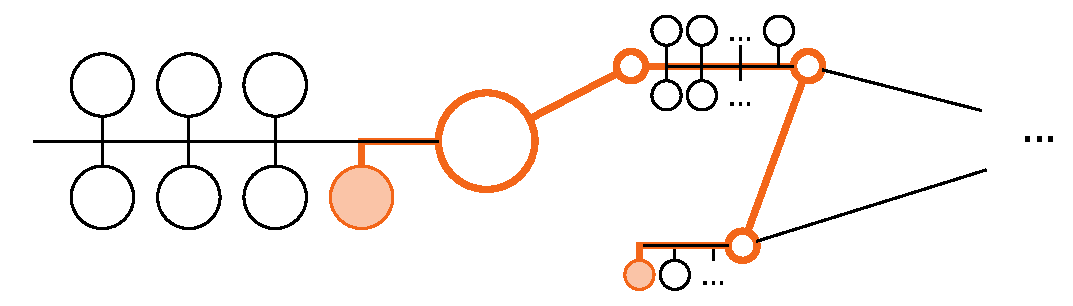
\includegraphics[width=\linewidth]{network_layer3.pdf}
\end{center}
\end{minipage}

\vspace{-0.75cm}


\subsection*{Capabilities}

The \conceptRef{IP}{Internet Protocol (IP)} allows exchanging \concept{datagrams} 
(Layer~3 \conceptRef{PDU}{PDUs}) between devices from different \conceptRef{LAN}{LANs}.
% 
Its addressing system identifies devices globally and makes it possible to 
\conceptRef{routing}{route} datagrams anywhere we need. 

Devices communicating via IP may belong to LANs
based on different technologies and with different types of \concept{MAC} address.
This has two implications:
\begin{itemize}
  \item A datagram that ``fits'' in the \concept{MTU} of the source LAN
    may be too large for the destination's (or any intermediate's) LAN MTU. 
    IP defines a \concept{fragmentation} system to split datagrams,
    which are reconstructed only at the final destination.\\[-0.25cm]
    
  \item When we send a datagram, we know the target device's \conceptRef{IP}{IP address},
  but not necessarily its \concept{MAC} address. Only if we are part of the destination
  LAN we will need that MAC. IP uses \concept{ARP} to translate known IP addresses
  to MAC addresses of the destination LAN's type.
\end{itemize}


\conceptRef{datagram}{Datagrams} may travel through networks not controlled 
by neither the source nor the destination, so datagrams may be lost, reordered and duplicated.
% 
Layer~3 does not provide mechanisms to deal with this; upper layers must implement
protection mechanisms when required 
(\eg, to implement \concept{TCP}'s \conceptRef{stream}{data streams}).

\begin{center}
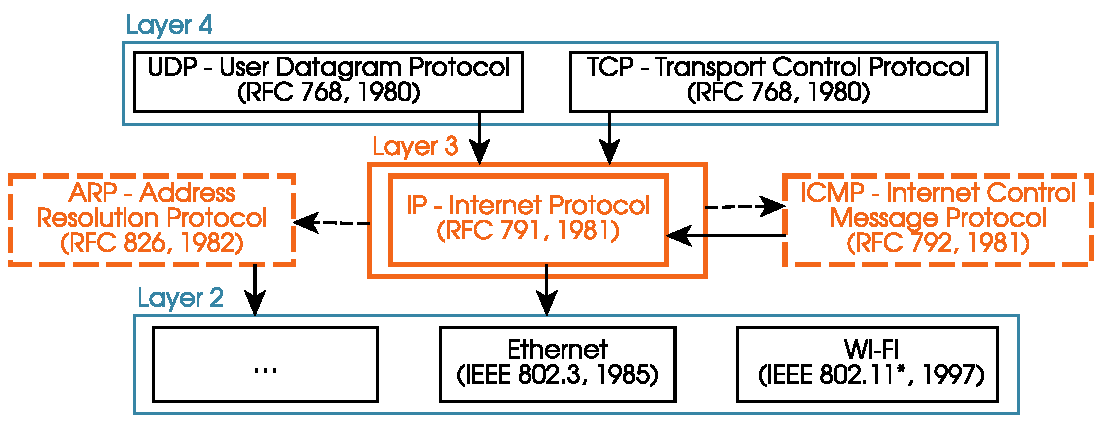
\includegraphics[width=0.9\linewidth]{protocols_layer3.pdf}
\end{center}


\vspace{-0.25cm}
\subsection*{Protocols}

Version~4 of \concept{IP} is \textit{the} protocol used in Layer~3, \ie,
it is common to virtually all communications in the Internet as we know it today.
% 
For many years, the Internet has been struggling to transition towards \concept{IPv6}, 
but the process is not complete and only \concept{IPv4} provides global coverage.

\concept{IPv4} delegates in the \concept{ARP} protocol the translation of known IP addresses 
into MAC addresses within each LAN. ARP does \textit{not} use IP datagrams.

The following protocols encapsulate their \conceptRef{PDU}{PDUs} in the payload of IP 
\conceptRef{datagram}{datagrams}:\\[-0.6cm]
\begin{itemize}
\item Transport Control Protocol (\concept{TCP}) 
\item User Datagram Protocol (\concept{UDP})
\item Internet Control Message Protocol (\concept{ICMP})
\end{itemize}

\begin{remark}
The \inlineCode{ip address}, \inlineCode{ip route} and \inlineCode{ip neighbor} commands 
(among others) let you query several aspects of your IP configuration.
\end{remark}



\section{Layer~3 Addressing}

\concept{IPv4} addresses are $32$~bit long. They are most often presented to humans in
the \concept{quad decimal} format, \eg, \otherBase{142.250.201.67}. 

\subsection*{Public and reserved addresses}

Most IP addresses are \conceptRef{public IP}{public} and unique across the Internet, 
\ie, the previous IP has the same meaning worldwide: it identifies a single connected device.
% 
Many addresses are \conceptRef{reserved IP address}{reserved/private} and can only be 
used within a particular scope (\eg, a LAN) or situation.
Some of the most common are the following (there are 
\href{https://en.wikipedia.org/wiki/Reserved_IP_addresses#IPv4}{\underline{some more}}):

\begin{center}
\begin{tabular}{ll}
\toprule
\textbf{IP address block} & \textbf{Address scope} \\
\toprule
\otherBase{127.*.*.*} & This computer (localhost) \\[0.1cm]
\otherBase{10.*.*.*} & This LAN \\
\otherBase{172.16.*.*} & This LAN \\
\otherBase{192.168.*.*} & This LAN \\[0.1cm]
\otherBase{0.*.*.*} & Special usages \\
\otherBase{169.254.*.*}& Special usages \\
\otherBase{255.255.255.255} & Special usages\\
\bottomrule
\end{tabular}
\end{center}

\begin{exercise}\ \\[-0.5cm]
\begin{itemize}
\item How many different \concept{IPv4} addresses are there (including reserved and private)? 
\item Are they sufficient now and in the future?
\item Is it problematic that an address like \otherBase{192.168.0.1} 
  is simultaneously used by thousands (likely millions) of computers in the Internet right now?
\end{itemize}
\end{exercise}

\subsection*{Netmasks}

The $32$~bits of an IP address can be divided in two parts using a \concept{netmask}:\\[-0.25cm]
% 
\begin{center}
\begin{bytefield}{32}
\bitheader{0-31}\\
\bitbox{10}{Network ID} & \bitbox{22}{Device ID} \\
\end{bytefield}
\end{center}
% 
The first part identifies the LAN or group of LANs to which a device belongs. 
The second part identifies a single device in the LAN. 
The netmask determines how many bits are assigned to each part. 

In the previous figure, the netmask assigns 10 bits to the network ID and 22 to the device ID.
This mask can be anywhere from $0$ (all bits are device ID) to $32$ (all bits are network ID).


Netmasks are presented to humans in two main ways:\\[-0.5cm]
\begin{itemize}
  \item \otherBase{/N}, where $N$ is the number of bits assigned to the Network ID. 
    This is used in the \concept{CIDR} format.
  
  \item The \concept{quad decimal} (\otherBase{A.B.C.D}) format of 
    $N$ bits set to \otherBase{1}, followed by $(32-N)$ bits set to \otherBase{0}.
\end{itemize}

\begin{exercise}
The netmask of the previous example can be expressed in binary 
(although it is not very convenient):
\begin{center}
\begin{bytefield}[bitwidth=1em]{32}
\bitheader{0-31} \\
\bitboxes{1}{1111111111} &
\bitboxes{1}{0000000000 0000000000 00} \\
\bitbox{10}{$10$~bits} & \bitbox{22}{$32-N = 22$~bits}
\end{bytefield}
\end{center}


\begin{itemize}
\item Express the netmask of the previous example in the CIDR and quad decimal formats.
\item What is your IP and netmask? Express it in the same two main ways.
\end{itemize}
\end{exercise}

\subsection*{Blocks of IP addresses}

Netmasks are used in combination with IP addresses to define 
\conceptRef{IP address block}{blocks of IP addresses} 
that begin with the same $N$ bits (where $N$ is the netmask).
% 
For instance, \otherBase{192.168.3.0/24} (in \concept{CIDR} format) 
and \otherBase{192.168.3.0/255.255.255.0} refer to the block 
of addresses between \otherBase{192.168.3.0} and \otherBase{192.168.3.255},
both included
(\otherBase{192.168.3.*} in the informal notation of the previous table).

\begin{exercise} 
IP blocks can be smaller than, equal to or larger than an IP network.
Provide examples where an IP block refers to:
\begin{itemize}
\item A single IP.
\item Half the IP addresses in the \otherBase{192.168.3.0/24} network.
\item All addresses of the \otherBase{192.168.3.0/24} network, plus 
      $256$ more addresses.
\item All possible IPs.
\end{itemize}
\end{exercise}


\begin{exercise}\ \\[-0.65cm]
\begin{itemize}
\item Can every \concept{netmask} be expressed as an \concept{IP address}?
\item List all possible netmasks.\\[-0.5cm]
\end{itemize}
\end{exercise}

When referring to a block of addresses (like a LAN), 
the IP address in this IP + netmask combination
must have all device ID bits set to \otherBase{0}. 
This way, \otherBase{192.168.3.0/24} correctly refers to a network, but
\otherBase{192.168.3.1/24} refers instead to a device 
(the one with IP \otherBase{192.168.3.1}) in that network (\otherBase{192.168.3.0/24}).

\begin{exercise}
\otherBase{192.168.0.0/24} $\ne$ \otherBase{192.168.0.0/25}. Why?
\end{exercise}

\subsection*{LANs and netmasks}

Netmasks need not be multiples of $8$. Consider the following example in which \\
\otherBase{192.168.76.1/19} (a device's IP + netmask) is used to obtain its network address\\
(\otherBase{192.168.64.0/19}):\\

\begin{center}
\begin{bytefield}[bitwidth=1.1em]{32}
\bitheader{0-31}\\
\begin{rightwordgroup}{Device's IP}
\bitbox{8}{192} & \bitbox{8}{168} & \bitbox{8}{76} &\bitbox{8}{1} \\
\bitboxes{1}{11000000} & \bitboxes{1}{10101000} & \bitboxes{1}{0100{\bf1}{\bf1}00} & \bitboxes{1}{0000000{\bf1}}
\end{rightwordgroup} \\

\bitboxes[]{1}{\&\&\&\& \&\&\&\& \&\&\&\& \&\&\&\& \&\&\&
               {\color{color1}\&} 
               {\color{color1}\&}{\color{color1}\&}{\color{color1}\&}{\color{color1}\&}
               {\color{color1}\&}{\color{color1}\&}{\color{color1}\&}{\color{color1}\&}
               {\color{color1}\&}{\color{color1}\&}{\color{color1}\&}{\color{color1}\&}} \\

\begin{rightwordgroup}{Netmask}
\bitboxes{1}{11111111111111111110000000000000}
\end{rightwordgroup} \\

\bitboxes[]{1}{==== ==== ==== ==== ===
               {\color{color1}=} 
               {\color{color1}=}{\color{color1}=}{\color{color1}=}{\color{color1}=}
               {\color{color1}=}{\color{color1}=}{\color{color1}=}{\color{color1}=}
               {\color{color1}=}{\color{color1}=}{\color{color1}=}{\color{color1}=}} \\

\begin{rightwordgroup}{Network IP}
\bitboxes{1}{11000000} & \bitboxes{1}{10101000} & \bitboxes{1}{0100{\bf0}{\bf0}00} & \bitboxes{1}{0000000{\bf0}} \\
\bitbox{8}{192} & \bitbox{8}{168} & \bitbox{8}{64} &\bitbox{8}{0} 
\end{rightwordgroup}\\
\end{bytefield}
\end{center}

\begin{exercise}\ \\[-0.5cm]
\begin{itemize}
\item In the previous example, we only really needed to transform one decimal value to binary,
and one decimal value to binary. Which one?
\item Is this always true when converting IP+netmask combinations to network addresses?
\item Express the netmask in \concept{quad decimal} format.
\end{itemize}
\end{exercise}



Given a IP + netmask address block and a device's IP address, it is direct to determine 
whether that device's IP belongs to the block (if and only if the first $N$ bits match,
where \otherBase{/N} is the CIDR netmask).

\begin{exercise}
Determine whether each of the following addresses belong to the same network as
the following device \otherBase{123.45.67.89/14}:
\begin{itemize}
\item \otherBase{23.45.67.89}
\item \otherBase{123.45.203.25}
\item \otherBase{123.43.255.255}
\item \otherBase{0.45.67.1}
\end{itemize}
\end{exercise}

An \conceptRef{network}{IP network} (a LAN) is a block of addresses, but not all those addresses 
can be assigned to devices. Two addresses are always reserved:
\begin{itemize}
\item The address with all node bits set to \otherBase{0}: it identifies the LAN itself.
\item The address with all node bits set to \otherBase{1}: it identifies \concept{broadcast} within the LAN.
\end{itemize}

\begin{exercise}\ \\[-0.5cm]
\begin{itemize}
\item List all addresses that can be assigned to devices in \otherBase{192.168.54.0/29}.
\item List the broadcast address of that network.
\end{itemize}
\end{exercise}

\begin{exercise}
The following code snippet takes an IP address and shows its $4$~bytes expressed in 
quad decimal and in binary.
Extend (or replace) the code so that you can:
\begin{itemize}
\item Transform $32$ bits into a quad decimal string
\item Display a netmask in IP address and CIDR formats
\item Given a device's IP and netmask, determine whether other IP belongs to the same network.
\end{itemize}
\begin{center}
\showCode{snippets/ipcalculator.py}
\end{center}
\end{exercise}




% \todo{exercise netmask calculator}
% 
% \todo{HERE HERE HERE: add and point to the subnetting area}







\section{IP -- Internet Protocol}

\subsection*{Packet format}

\concept{IP} defines a \concept{packet} format with a \concept{header} 
that is \textit{at least} $20$~bytes long. Optional parts may be included,
as long as the total header size is a multiple of $32$~bits ($4$~bytes).
The payload can be empty, so the minimum datagram size is $20$~bytes.\\

\begin{center}
\small
\begin{bytefield}[bitheight=3.4em,bitwidth=1.1em]{32}
\bitheader{0-31}\\
\begin{rightwordgroup}[curlyshrinkage=10pt]{Mandatory Header\\($20$~bytes)}
  \bitbox{4}{IP\\Version} 
  & \bitbox{4}{IHL\\{\scriptsize(HLen/$4$)}} 
  & \bitbox{8}[bgcolor=lightgray]{Type of Service}
  & \bitbox{16}{Datagram Length\\{\scriptsize(Head + Payload, bytes)}} \\
  % 
  \bitbox{16}{Fragment ID} & \bitbox{1}{\otherBase{0}}
  & \bitbox{1}{\rotatebox{90}{\scriptsize DF flag}}
  & \bitbox{1}{\rotatebox{90}{\scriptsize MF flag}}
  & \bitbox{13}{Fragment Offset} \\
  % 
  \bitbox{8}{Time to Live\\(TTL)}
  & \bitbox{8}{Payload protocol}
  & \bitbox{16}[bgcolor=lightgray]{IP Header Checksum}\\
  % 
  \bitbox{32}{Source IP Address} \\
  \bitbox{32}{Destination IP Address}
\end{rightwordgroup} \\
%   
\begin{rightwordgroup}[curlyshrinkage=10pt]{Optional Header\\{\scriptsize($4x$~bytes)}}
\bitbox[tlr]{32}[bgcolor=lightgray]{Options\\{\scriptsize(variable length, optional)}} \\
\bitbox[lbr]{24}[bgcolor=lightgray]{} &
\bitbox{8}[bgcolor=lightgray]{Padding to\\$32$ bits}
\end{rightwordgroup} \\
% 
\begin{rightwordgroup}[curlyshrinkage=10pt]{Payload\\{\scriptsize($y$~bytes)}}
\bitbox[tlr]{32}{Payload data} \\
\bitbox[lbr]{8}{} & \bitbox[t]{24}{} 
\end{rightwordgroup}
\end{bytefield}
\end{center}

\begin{exercise} \ \\[-0.5cm]
\begin{itemize}
\item How can the payload length be calculated from the header?
\item What is the maximum payload length?
\item What are the possible values of the flags in the IP header?
\item What's longer, an IP address or an Ethernet MAC address?
\item Is it possible to send exactly 17 bits of payload data in an IP datagram?
\item How can we know whether a datagram is encapsulating TCP or UDP data?
\item Why must the optional header part by a multiple of $32$~bits?
\end{itemize}
\end{exercise}

\subsection*{Operation}

When a device A wants to send an IP datagram to a device B, the source and 
destination IPs in the header are fixed and don't change for this datagram.

If devices A and B belong to the same LAN, the datagram is sent directly
(\eg, encapsulated in an Ethernet frame). However, IP can go much farther.
Consider the following scenario, where A wants to communicate with D.

\begin{center}
 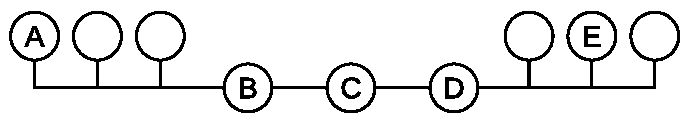
\includegraphics[width=0.5\linewidth]{ip_operation_example.pdf}
\end{center}


Here, the source and destination devices belong to different LANs.
The datagram is passed first to the source's \conceptRef{router}{gateway router}. 
Then, each intermediate router passes it to the next one until the datagram reaches 
the last router, which is connected to the destination LAN. Finally, that last router 
passes the datagram to the destination. 

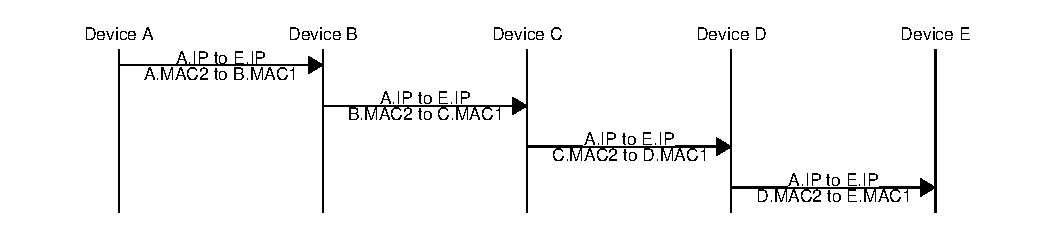
\includegraphics{ip_operation.eps}


The source and destination IP addresses don't change throughout the journey.
In contrast, MAC address change in each LAN \concept{hop}. 

\begin{remark}
In this example, the gateway router~(B) is directly connected to the destination LAN's router~(C).
Normally, there would be several routers chained between B and C.
\end{remark}







% \subsection{IP addresses, netmasks and CIDR format}\label{sec:layer3:cidr}
% also division
% 
% \subsection{Fragmentation}
% 
% \subsection{Routing}

\section{ARP -- Address Resolution Protocol}
\begin{remark}
The \concept{ARP} protocol does \textit{not} use IP headers.
\end{remark}

\section{ICMP -- Internet Control Message Protocol}


% - talk about the problem of having different networks, different technologoies (ARPA, XEROX
% - longest prefix matching for routing tables
% - first draft: 8-bit network addresses (a bit off!)
